%!TEX program = pdflatex
%----------------------------------------------------------------------------------------
% TEMPLATE INFORMATON
%----------------------------------------------------------------------------------------
% This template was adapted from "The Legrand Orange Book Version 1.4 (12/4/14) [http://www.LaTeXTemplates.com] Mathias Legrand (legrand.mathias@gmail.com)" License: CC BY-NC-SA 3.0 (http://creativecommons.org/licenses/by-nc-sa/3.0/)
%----------------------------------------------------------------------------------------

%----------------------------------------------------------------------------------------
% COMPILACAO
%----------------------------------------------------------------------------------------
% 0) There is a "compilar.sh"
% OR
% 1) pdflatex livro_algoritmos_e_estruturas_de_dados
% 2) makeindex livro_algoritmos_e_estruturas_de_dados.idx -s StyleInd.ist
% 3) biber livro_algoritmos_e_estruturas_de_dados
% 4) pdflatex livro_algoritmos_e_estruturas_de_dados
% 5) pdflatex livro_algoritmos_e_estruturas_de_dados

%----------------------------------------------------------------------------------------
%	PACKAGES AND OTHER DOCUMENT CONFIGURATIONS
%----------------------------------------------------------------------------------------
\documentclass[11pt,fleqn]{book} % Default font size and left-justified equations

%encoding
%--------------------------------------
\usepackage[T1]{fontenc}
%--------------------------------------
\usepackage[utf8]{inputenc}
\hyphenation{Mi-nis-té-ri-o}
\usepackage[top=3cm,bottom=3cm,left=3.2cm,right=3.2cm,headsep=10pt,a4paper]{geometry} % Page margins
\usepackage[svgnames]{xcolor} % Required for specifying colors by name
\definecolor{blue}{rgb}{0.0, 0.18, 0.39}
% Font Settings
\usepackage{avant} % Use the Avantgarde font for headings
%\usepackage{times} % Use the Times font for headings
\usepackage{mathptmx} % Use the Adobe Times Roman as the default text font together with math symbols from the Sym­bol, Chancery and Com­puter Modern fonts
\usepackage{microtype} % Slightly tweak font spacing for aesthetics
% Index
\usepackage{calc} % For simpler calculation - used for spacing the index letter headings correctly
\usepackage{makeidx} % Required to make an index
\makeindex % Tells LaTeX to create the files required for indexing
\usepackage{verbatim}
% Others
\usepackage[colorinlistoftodos,prependcaption,textsize=tiny,linecolor=red,backgroundcolor=red!25,bordercolor=red]{todonotes}
\usepackage{epigraph}
\renewcommand{\textflush}{flushepinormal}
\setlength{\epigraphwidth}{0.8\textwidth}

\usepackage{nameref}
\usepackage{booktabs}
\usepackage{graphicx}
\usepackage{float}
\usepackage{multirow}

%CODE
\usepackage{courier}
\usepackage{listings}
\lstset{
	numbers=left,                   % where to put the line-numbers
	stepnumber=1,                   % the step between two line-numbers. 	
	frame=tb,                       % draw a frame at the top and bottom of the code block
	tabsize=4,                      % tab space width
	showstringspaces=false,         % don't mark spaces in strings
	numbers=left,                   % display line numbers on the left
	commentstyle=\color{Gray},      % comment color
	keywordstyle=\color{DarkBlue},  % keyword color
	stringstyle=\color{Maroon},     % string color
	breaklines=true,                % break lines when it's needed
	basicstyle=\ttfamily\scriptsize % font family and size (need package courier)
}
\renewcommand{\lstlistingname}{Programa}

% Bibliography
%\usepackage[backend=biber,style=authoryear,autocite=inline, citestyle=authoryear]{biblatex}
\usepackage[style=abnt]{biblatex}
\addbibresource{bibliography.bib} % BibTeX bibliography file
\defbibheading{bibempty}{}
\renewcommand*{\nameyeardelim}{\addcomma\space}

\newcommand{\VER}[1]{\begingroup\color{red}#1\endgroup}

%----------------------------------------------------------------------------------------

%----------------------------------------------------------------------------------------
%	VARIOUS REQUIRED PACKAGES
%----------------------------------------------------------------------------------------
%--------------------------------------
\usepackage[brazil,english]{babel}
%\usepackage[english,brazil]{babel} % English language/hyphenation
%--------------------------------------
\usepackage{titlesec} % Allows customization of titles
%--------------------------------------
\usepackage{graphicx} % Required for including pictures
\graphicspath{{Pictures/}} % Specifies the directory where pictures are stored
%--------------------------------------
\usepackage{lipsum} % Inserts dummy text
%--------------------------------------
\usepackage{tikz} % Required for drawing custom shapes
%--------------------------------------
\usepackage{enumitem} % Customize lists
\setlist{nolistsep} % Reduce spacing between bullet points and numbered lists
%--------------------------------------
\usepackage{booktabs} % Required for nicer horizontal rules in tables
%--------------------------------------
\usepackage{eso-pic} % Required for specifying an image background in the title page
%--------------------------------------

%----------------------------------------------------------------------------------------
%	MAIN TABLE OF CONTENTS
%----------------------------------------------------------------------------------------

\usepackage{titletoc} % Required for manipulating the table of contents

\contentsmargin{0cm} % Removes the default margin
% Chapter text styling
\titlecontents{chapter}[1.25cm] % Indentation
{\addvspace{15pt}\large\sffamily\bfseries} % Spacing and font options for chapters
{\color{blue!60}\contentslabel[\Large\thecontentslabel]{1.25cm}\color{blue}} % Chapter number
{}  
{\color{blue!60}\normalsize\sffamily\bfseries\;\titlerule*[.5pc]{.}\;\thecontentspage} % Page number
% Section text styling
\titlecontents{section}[1.25cm] % Indentation
{\addvspace{5pt}\sffamily\bfseries} % Spacing and font options for sections
{\contentslabel[\thecontentslabel]{1.25cm}} % Section number
{}
{\sffamily\hfill\color{black}\thecontentspage} % Page number
[]
% Subsection text styling
\titlecontents{subsection}[1.25cm] % Indentation
{\addvspace{15pt}\sffamily\small} % Spacing and font options for subsections
{\contentslabel[\thecontentslabel]{1.25cm}} % Subsection number
{}
{\sffamily\;\titlerule*[.5pc]{.}\;\thecontentspage} % Page number
[] 

%----------------------------------------------------------------------------------------
%	MINI TABLE OF CONTENTS IN CHAPTER HEADS
%----------------------------------------------------------------------------------------

% Section text styling
\titlecontents{lsection}[.05em] % Indendating
{\footnotesize\sffamily} % Font settings
{}
{}
{}

% Subsection text styling
\titlecontents{lsubsection}[.5em] % Indentation
{\normalfont\footnotesize\sffamily} % Font settings
{}
{}
{}
 
%----------------------------------------------------------------------------------------
%	PAGE HEADERS
%----------------------------------------------------------------------------------------

\usepackage{fancyhdr} % Required for header and footer configuration

\pagestyle{fancy}
\renewcommand{\chaptermark}[1]{\markboth{\sffamily\normalsize\bfseries\chaptername\ \thechapter.\ #1}{}} % Chapter text font settings
\renewcommand{\sectionmark}[1]{\markright{\sffamily\normalsize\thesection\hspace{10pt}#1}{}} % Section text font settings
\fancyhf{} \fancyhead[LE,RO]{\sffamily\normalsize\thepage} % Font setting for the page number in the header
\fancyhead[LO]{\rightmark} % Print the nearest section name on the left side of odd pages
\fancyhead[RE]{\leftmark} % Print the current chapter name on the right side of even pages
\renewcommand{\headrulewidth}{0.5pt} % Width of the rule under the header
\addtolength{\headheight}{2.5pt} % Increase the spacing around the header slightly
\renewcommand{\footrulewidth}{0pt} % Removes the rule in the footer
\fancypagestyle{plain}{\fancyhead{}\renewcommand{\headrulewidth}{0pt}} % Style for when a plain pagestyle is specified

% Removes the header from odd empty pages at the end of chapters
\makeatletter
\renewcommand{\cleardoublepage}{
\clearpage\ifodd\c@page\else
\hbox{}
\vspace*{\fill}
\thispagestyle{empty}
\newpage
\fi}

%----------------------------------------------------------------------------------------
%	THEOREM STYLES
%----------------------------------------------------------------------------------------

\usepackage{amsmath,amsfonts,amssymb,amsthm} % For math equations, theorems, symbols, etc

\newcommand{\intoo}[2]{\mathopen{]}#1\,;#2\mathclose{[}}
\newcommand{\ud}{\mathop{\mathrm{{}d}}\mathopen{}}
\newcommand{\intff}[2]{\mathopen{[}#1\,;#2\mathclose{]}}
\newtheorem{notation}{Notation}[chapter]

%%%%%%%%%%%%%%%%%%%%%%%%%%%%%%%%%%%%%%%%%%%%%%%%%%%%%%%%%%%%%%%%%%%%%%%%%%%
%%%%%%%%%%%%%%%%%%%% dedicated to boxed/framed environements %%%%%%%%%%%%%%
%%%%%%%%%%%%%%%%%%%%%%%%%%%%%%%%%%%%%%%%%%%%%%%%%%%%%%%%%%%%%%%%%%%%%%%%%%%
\newtheoremstyle{bluenumbox}% % Theorem style name
{0pt}% Space above
{0pt}% Space below
{\normalfont}% % Body font
{}% Indent amount
{\small\bf\sffamily\color{blue}}% % Theorem head font
{\;}% Punctuation after theorem head
{0.25em}% Space after theorem head
{\small\sffamily\color{blue}\thmname{#1}\nobreakspace\thmnumber{\@ifnotempty{#1}{}\@upn{#2}}% Theorem text (e.g. Theorem 2.1)
\thmnote{\nobreakspace\the\thm@notefont\sffamily\bfseries\color{black}---\nobreakspace#3.}} % Optional theorem note
\renewcommand{\qedsymbol}{$\blacksquare$}% Optional qed square

\newtheoremstyle{blacknumex}% Theorem style name
{5pt}% Space above
{5pt}% Space below
{\normalfont}% Body font
{} % Indent amount
{\small\bf\sffamily}% Theorem head font
{\;}% Punctuation after theorem head
{0.25em}% Space after theorem head
{\small\sffamily{\tiny\ensuremath{\blacksquare}}\nobreakspace\thmname{#1}\nobreakspace\thmnumber{\@ifnotempty{#1}{}\@upn{#2}}% Theorem text (e.g. Theorem 2.1)
\thmnote{\nobreakspace\the\thm@notefont\sffamily\bfseries---\nobreakspace#3.}}% Optional theorem note

\newtheoremstyle{blacknumbox} % Theorem style name
{0pt}% Space above
{0pt}% Space below
{\normalfont}% Body font
{}% Indent amount
{\small\bf\sffamily}% Theorem head font
{\;}% Punctuation after theorem head
{0.25em}% Space after theorem head
{\small\sffamily\thmname{#1}\nobreakspace\thmnumber{\@ifnotempty{#1}{}\@upn{#2}}% Theorem text (e.g. Theorem 2.1)
\thmnote{\nobreakspace\the\thm@notefont\sffamily\bfseries---\nobreakspace#3.}}% Optional theorem note

%%%%%%%%%%%%%%%%%%%%%%%%%%%%%%%%%%%%%%%%%%%%%%%%%%%%%%%%%%%%%%%%%%%%%%%%%%%
%%%%%%%%%%%%% dedicated to non-boxed/non-framed environements %%%%%%%%%%%%%
%%%%%%%%%%%%%%%%%%%%%%%%%%%%%%%%%%%%%%%%%%%%%%%%%%%%%%%%%%%%%%%%%%%%%%%%%%%
\newtheoremstyle{bluenum}% % Theorem style name
{5pt}% Space above
{5pt}% Space below
{\normalfont}% % Body font
{}% Indent amount
{\small\bf\sffamily\color{blue}}% % Theorem head font
{\;}% Punctuation after theorem head
{0.25em}% Space after theorem head
{\small\sffamily\color{blue}\thmname{#1}\nobreakspace\thmnumber{\@ifnotempty{#1}{}\@upn{#2}}% Theorem text (e.g. Theorem 2.1)
\thmnote{\nobreakspace\the\thm@notefont\sffamily\bfseries\color{black}---\nobreakspace#3.}} % Optional theorem note
\renewcommand{\qedsymbol}{$\blacksquare$}% Optional qed square
\makeatother

% Defines the theorem text style for each type of theorem to one of the three styles above
\newcounter{dummy} 
\numberwithin{dummy}{section}
\theoremstyle{bluenumbox}
\newtheorem{theoremeT}[dummy]{Theorem}
\newtheorem{problem}{Problem}[chapter]
\newtheorem{exerciseT}{Exercise}[chapter]
\theoremstyle{blacknumex}
\newtheorem{exampleT}{Example}[chapter]
\theoremstyle{blacknumbox}
\newtheorem{vocabulary}{Vocabulary}[chapter]
\newtheorem{definitionT}{Definition}[section]
\newtheorem{corollaryT}[dummy]{Corollary}
\theoremstyle{bluenum}
\newtheorem{proposition}[dummy]{Proposition}

%----------------------------------------------------------------------------------------
%	DEFINITION OF COLORED BOXES
%----------------------------------------------------------------------------------------

\RequirePackage[framemethod=default]{mdframed} % Required for creating the theorem, definition, exercise and corollary boxes

% Theorem box
\newmdenv[skipabove=7pt,
skipbelow=7pt,
backgroundcolor=black!5,
linecolor=blue,
innerleftmargin=5pt,
innerrightmargin=5pt,
innertopmargin=5pt,
leftmargin=0cm,
rightmargin=0cm,
innerbottommargin=5pt]{tBox}

% Exercise box	  
\newmdenv[skipabove=7pt,
skipbelow=7pt,
rightline=false,
leftline=true,
topline=false,
bottomline=false,
backgroundcolor=blue!10,
linecolor=blue,
innerleftmargin=5pt,
innerrightmargin=5pt,
innertopmargin=5pt,
innerbottommargin=5pt,
leftmargin=0cm,
rightmargin=0cm,
linewidth=4pt]{eBox}	

% Definition box
\newmdenv[skipabove=7pt,
skipbelow=7pt,
rightline=false,
leftline=true,
topline=false,
bottomline=false,
linecolor=blue,
innerleftmargin=5pt,
innerrightmargin=5pt,
innertopmargin=0pt,
leftmargin=0cm,
rightmargin=0cm,
linewidth=4pt,
innerbottommargin=0pt]{dBox}	

% Corollary box
\newmdenv[skipabove=7pt,
skipbelow=7pt,
rightline=false,
leftline=true,
topline=false,
bottomline=false,
linecolor=gray,
backgroundcolor=black!5,
innerleftmargin=5pt,
innerrightmargin=5pt,
innertopmargin=5pt,
leftmargin=0cm,
rightmargin=0cm,
linewidth=4pt,
innerbottommargin=5pt]{cBox}

% Creates an environment for each type of theorem and assigns it a theorem text style from the "Theorem Styles" section above and a colored box from above
\newenvironment{theorem}{\begin{tBox}\begin{theoremeT}}{\end{theoremeT}\end{tBox}}
\newenvironment{exercise}{\begin{eBox}\begin{exerciseT}}{\hfill{\color{blue}\tiny\ensuremath{\blacksquare}}\end{exerciseT}\end{eBox}}				  
\newenvironment{definition}{\begin{dBox}\begin{definitionT}}{\end{definitionT}\end{dBox}}	
\newenvironment{example}{\begin{exampleT}}{\hfill{\tiny\ensuremath{\blacksquare}}\end{exampleT}}		
\newenvironment{corollary}{\begin{cBox}\begin{corollaryT}}{\end{corollaryT}\end{cBox}}	

%----------------------------------------------------------------------------------------
%	REMARK ENVIRONMENT
%----------------------------------------------------------------------------------------

\newenvironment{remark}{\par\vspace{10pt}\small % Vertical white space above the remark and smaller font size
\begin{list}{}{
\leftmargin=35pt % Indentation on the left
\rightmargin=25pt}\item\ignorespaces % Indentation on the right
\makebox[-2.5pt]{\begin{tikzpicture}[overlay]
\node[draw=blue!60,line width=1pt,circle,fill=blue!25,font=\sffamily\bfseries,inner sep=2pt,outer sep=0pt] at (-15pt,0pt){\textcolor{blue}{R}};\end{tikzpicture}} % Orange R in a circle
\advance\baselineskip -1pt}{\end{list}\vskip5pt} % Tighter line spacing and white space after remark

%----------------------------------------------------------------------------------------
%	SECTION NUMBERING IN THE MARGIN
%----------------------------------------------------------------------------------------

\makeatletter
\renewcommand{\@seccntformat}[1]{\llap{\textcolor{blue}{\csname the#1\endcsname}\hspace{1em}}}                    
\renewcommand{\section}{\@startsection{section}{1}{\z@}
{-4ex \@plus -1ex \@minus -.4ex}
{1ex \@plus.2ex }
{\normalfont\large\sffamily\bfseries}}
\renewcommand{\subsection}{\@startsection {subsection}{2}{\z@}
{-3ex \@plus -0.1ex \@minus -.4ex}
{0.5ex \@plus.2ex }
{\normalfont\sffamily\bfseries}}
\renewcommand{\subsubsection}{\@startsection {subsubsection}{3}{\z@}
{-2ex \@plus -0.1ex \@minus -.2ex}
{.2ex \@plus.2ex }
{\normalfont\small\sffamily\bfseries}}                        
\renewcommand\paragraph{\@startsection{paragraph}{4}{\z@}
{-2ex \@plus-.2ex \@minus .2ex}
{.1ex}
{\normalfont\small\sffamily\bfseries}}

%----------------------------------------------------------------------------------------
%	HYPERLINKS IN THE DOCUMENTS
%----------------------------------------------------------------------------------------

% For an unclear reason, the package should be loaded now and not later
\usepackage{hyperref}
\hypersetup{hidelinks,backref=true,pagebackref=true,hyperindex=true,colorlinks=true,breaklinks=true,urlcolor= DarkBlue,linkcolor=DarkBlue,bookmarks=true,bookmarksopen=false,pdftitle={Title},pdfauthor={Author}}

%----------------------------------------------------------------------------------------
%	CHAPTER HEADINGS
%----------------------------------------------------------------------------------------

% The set-up below should be (sadly) manually adapted to the overall margin page septup controlled by the geometry package loaded in the main.tex document. It is possible to implement below the dimensions used in the goemetry package (top,bottom,left,right)... TO BE DONE

\newcommand{\thechapterimage}{}
\newcommand{\chapterimage}[1]{\renewcommand{\thechapterimage}{#1}}

% Numbered chapters with mini tableofcontents
\def\thechapter{\arabic{chapter}}
\def\@makechapterhead#1{
\thispagestyle{empty}
{\centering \normalfont\sffamily
\ifnum \c@secnumdepth >\m@ne
\if@mainmatter
\startcontents
\begin{tikzpicture}[remember picture,overlay]
\node at (current page.north west)
{\begin{tikzpicture}[remember picture,overlay]
\node[rounded corners=5pt,anchor=north west,inner sep=0pt] at (0,0) {\includegraphics[width=\paperwidth]{\thechapterimage}};
%%%%%%%%%%%%%%%%%%%%%%%%%%%%%%%%%%%%%%%%%%%%%%%%%%%%%%%%%%%%%%%%%%%%%%%%%%%%%%%%%%%%%
%Tamanho do mini table of contents
\fill[color=blue!10!white,opacity=.6] (.5cm,0) rectangle (9.9cm,-13cm);
%Conteúdo do mini table of contents 
\node[rounded corners=10pt,anchor=north west] at (1.1cm,.35cm) {\parbox[t][10cm][t]{10cm}{\huge\bfseries\flushleft \printcontents{l}{1}{\setcounter{tocdepth}{2}}}};
%Titulo do capitulo
\draw[anchor=west] (10cm,-10cm) node [rounded corners=5pt,fill=blue!10!white,text opacity=1,draw=blue,draw opacity=1,line width=1.5pt,fill opacity=.6,inner sep=12pt]{\huge\sffamily\bfseries\textcolor{black}{\thechapter. #1\strut\makebox[20cm]{}}};
%%%%%%%%%%%%%%%%%%%%%%%%%%%%%%%%%%%%%%%%%%%%%%%%%%%%%%%%%%%%%%%%%%%%%%%%%%%%%%%%%%%%%
\end{tikzpicture}};
\end{tikzpicture}}
\par\vspace*{230\p@}
\fi
\fi}

% Unnumbered chapters without mini tableofcontents (could be added though) 
\def\@makeschapterhead#1{
\thispagestyle{empty}
{\centering \normalfont\sffamily
\ifnum \c@secnumdepth >\m@ne
\if@mainmatter
\begin{tikzpicture}[remember picture,overlay]
\node at (current page.north west)
{\begin{tikzpicture}[remember picture,overlay]
\node[anchor=north west,inner sep=0pt] at (0,0) {\includegraphics[width=\paperwidth]{\thechapterimage}};
\draw[anchor=west] (2cm,-9cm) node [rounded corners=5pt,fill=blue!10!white,fill opacity=.6,inner sep=12pt,text opacity=1,draw=blue,draw opacity=1,line width=1.5pt]{\huge\sffamily\bfseries\textcolor{black}{#1\strut\makebox[22cm]{}}};
\end{tikzpicture}};
\end{tikzpicture}}
\par\vspace*{230\p@}
\fi
\fi
}
\makeatother % Insert the commands.tex file which contains the majority of the structure behind the template

\begin{document}

\let\cleardoublepage\clearpage

\renewcommand{\chaptername}{Capítulo}
\renewcommand{\figurename}{Fig.}

%----------------------------------------------------------------------------------------
%	TITLE PAGE
%----------------------------------------------------------------------------------------
\begingroup
	\thispagestyle{empty}
	
	\AddToShipoutPicture*{\put(0,0){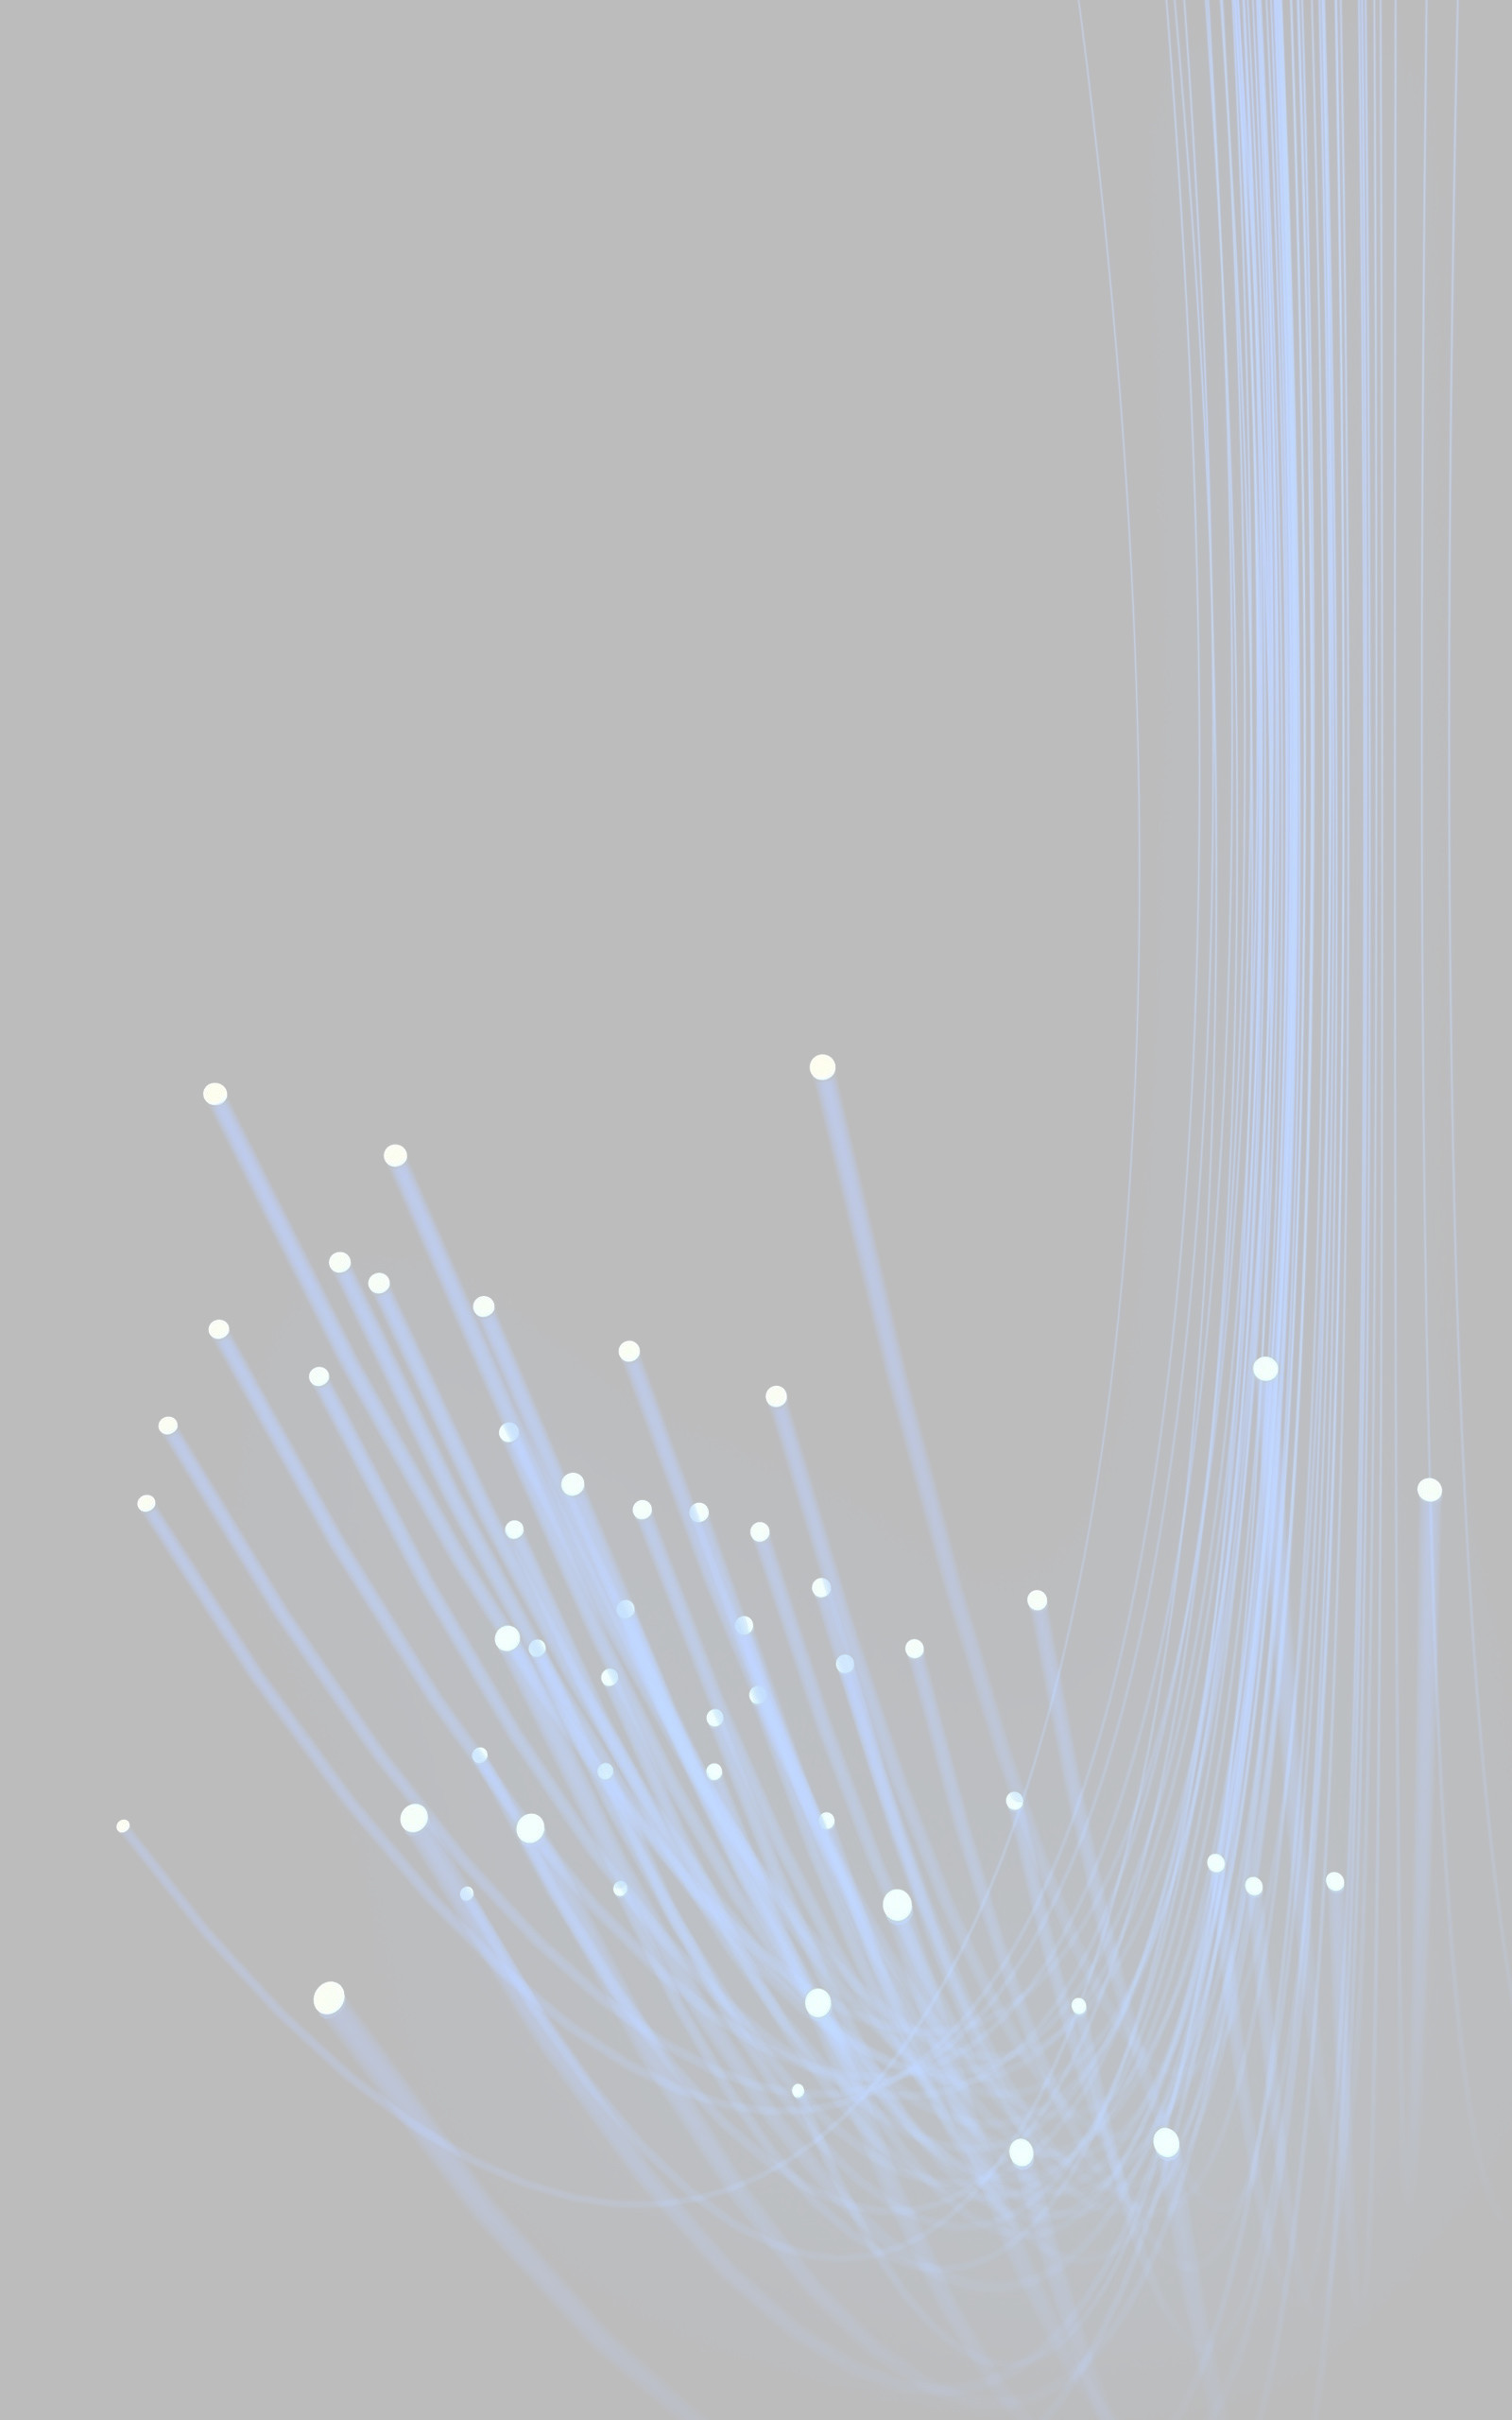
\includegraphics[scale=1]{capa}}} % Image background
	
	%\AddToShipoutPicture*{\put(116,650){
\includegraphics[scale=.75]{brasao.png}}} % Image background
	
	%\AddToShipoutPicture*{\put(244,200){
\includegraphics[scale=0.2]{ifgvertical}}} % Image background
	\AddToShipoutPicture*{\put(244,650){
\includegraphics[scale=0.2]{ifgvertical}}} % Image background
	
	\vspace*{4.5cm}
	
	\centering
	\par
	\fontsize{30}{30}
	\selectfont
	Algoritmos e Estruturas de Dados \\
	\vspace*{1.5cm}
	\par
	\fontsize{16}{16}
	\selectfont
	Tecnólogo em Análise e Desenvolvimento de Sistemas\\
	\vspace*{1.5cm}
	Waldeyr Mendes Cordeiro da Silva\\
	\vspace*{10cm}
	\par
	{\Huge 2019}
	\par
\endgroup
\pagebreak

%----------------------------------------------------------------------------------------
%	PEOPLE PAGE
%----------------------------------------------------------------------------------------
\chapterimage{banner3} % Chapter heading image
\par
\section*{Material didático para Algoritmos e Estruturas de Dados}

Versão 0.1

\section*{Waldeyr Mendes Cordeiro da Silva}\label{WaldeyrMendes}
\begin{itemize}
	\item Formação:
	\begin{itemize}
		\item Bacharelado em Sistemas de Informação
		\item Licenciatura em Ciências Biológicas
		\item Complementação Pedagógica em Matemática
		\item Especialização em Engenharia de Software
		\item Especialização em Segurança da Informação
		\item Mestrado em Informática
		\item Doutorado em Ciências Biológicas (Bioinformática)
	\end{itemize}
	\item 
\includegraphics[scale=.03]{Pictures/lattes}~\href{http://lattes.cnpq.br/2391349697609978}{Lattes: http://lattes.cnpq.br/2391349697609978}
	\item 
\includegraphics[scale=.15]{Pictures/orcid}~\href{https://orcid.org/0000-0002-8660-6331}{ORCID: https://orcid.org/0000-0002-8660-6331}
\end{itemize}

\chapterimage{banner3} % Chapter heading image
\renewcommand\contentsname{Sumário}
\tableofcontents

%----------------------------------------------------------------------------------------
%	CHAPTER
%----------------------------------------------------------------------------------------
\chapterimage{01.jpg} % Chapter heading image
\chapter{Prefácio}\label{prefacio}
\vspace{6em}
\begin{flushright}
	\textit{\textcolor{white}{Um bonita citação...}}
\end{flushright}
\vspace{12em}

\todo[inline]{Em construção...}

Este livro destina-se aos acadêmicos e demais interessados em iniciar os estudos em algoritmos e estruturas de dados.

%----------------------------------------------------------------------------------------
%	CHAPTER
%----------------------------------------------------------------------------------------
\chapterimage{02.jpg} % Chapter heading image
\chapter{Introdução}\label{introducao}
\vspace{6em}
\begin{flushright}
	\textit{\textcolor{white}{Um bonita citação...}}
\end{flushright}
\vspace{12em}


Um algoritmo é um procedimento computacional bem definido que processa um valor ou um conjunto de dados (entrada) e produz algum valor ou conjunto de dados (saída)~\cite{cormen2009}.
Os algoritmos existem há muito tempo, mas estão presentes na sociedade moderna de uma forma nunca experimentada na história da humanidade.
Quase tudo que se produz, sejam produtos ou serviços, tem alguma influência de algoritmos.
O comércio eletrônico utiliza tanto algoritmos clássicos como ordenações, quanto algoritmos modernos de recomendação de produtos baseado no histórico de visitas.
A segurança das senhas em qualquer sistema bancário ou \textit{Web} é garantida por algoritmos de criptografia.
Imagens de satélite, dados genômicos, reconhecimento de faces, previsão do tempo, quase tudo que se possa imaginar atualmente é influenciado direta oou indiretamente por algum algoritmo.

O estudo de algoritmos é uma demanda crescente frente aos novos desafios trazidos pelo grande volume de dados que as tecnologias modernas proporcionaram.
A análise de algortimos é uma área com questões importantes em aberto, como é o caso dos \textit{Millennium Prize Problems}, com sete problemas matemático-computacionais em aberto e cujo prêmio é de 1 milhão de dólares por cada solução.

O propósito da análise de um algortimo é prever seu comportamento quanto ao tempo de execução ou ao espaço em memória que irá ocupar mesmo antes de ser executado em um computador específico.
Porém, muitos fatores, como o tamanho e a variedade dos dos dados de entrada, influenciam o algoritmo.
Portanto, a análise de algoritmos provê uma aproximação, o que em muitos casos é bastante significante.

Tipos abstratos de dados são conjuntos de valores sobre os quais é possível aplicar funções de forma homogênea através de um algortimo.
Funções e valores em conjunto, consituem um modelo matemático que pode ser empregado em problemas do mundo real~\cite{ascencio2010}.
Os algortimos são projetados em função de um tipo abstrato de dados.
A representação computacional de um tipo abstrato de dados com seus tipos e operações permitidas pode ser entendida como uma \textbf{estrutura de dados}.
Uma estrutura de dados é um meio para aramzenar e processar dados com vistas à sua organização, acesso e modificações~\cite{cormen2009}.

\section{Análise de Algoritmos}\label{sec_analise}

\subsection{Elementos de Notação Assintótica}




%----------------------------------------------------------------------------------------
%	CHAPTER
%----------------------------------------------------------------------------------------
%------------------------------------------------
\chapterimage{04.jpg} % Chapter heading image
\chapter{Programação}\label{programacao}
\vspace{6em}
\begin{flushright}
	\textit{\textcolor{white}{Um bonita citação...}}
\end{flushright}
\vspace{12em}



\newpage
\section{Primeiros Passos em Programação}\label{disc:primeirospassos}

\lstinputlisting[language=C, caption={Meu primeiro programa em C.}]{Code/Basics/prog001.c}\label{prog001}



%----------------------------------------------------------------------------------------
%	CHAPTER X
%----------------------------------------------------------------------------------------
%------------------------------------------------
\chapterimage{05.jpg} % Chapter heading image
\chapter{Estruturas de Dados}\label{estrutura}
\vspace{6em}
\begin{flushright}
	\textit{\textcolor{white}{Um bonita citação...}}
\end{flushright}
\vspace{12em}

\newpage
\section{Estruturas de Dados Homogêneas e Heterogêneas}\label{tipos}

\subsection*{Vetores}

Primeiro, uma revisão sobre vetores.
Em C uma variável que represente um vetor é um ponteiro.
Portanto, quando um vetor é parâmetro para uma função o que é passado é a sua referência, ou seja, o endereço base do vetor.
Vetores podem ser bi-, tri-, ou multi-domensionais, mas abrigam o mesmo tipo de dados.
O programa~\ref{rev001} mostra o vetor sendo passado para uma função que retorna o valor do meio do vetor.

\lstinputlisting[language=C, caption={Em C, vetores são passados para funções por referência.}]{Code/Revisao/rev001.c}\label{rev001}

\lstinputlisting[language=C, caption={Um vetor de duas dimensões mostrando apenas valores da diagonal principal.}]{Code/Revisao/rev003.c}\label{rev003}

\subsection*{Strings em C}
Em C, uma \textit{string} é um vetor de caracteres e cada \textit{string} termina com um caracter \textit{NULL}.
Uma constante \textit{string} é definida dentro de aspas em que o caractere \textit{NULL} é automaticamente incluído.
Por exemplo, a string "IFG" é um vetor de 4 elementos.
O programa~\ref{rev002} mostra um exemplo de \textit{string} em C. 
\lstinputlisting[language=C, caption={Em C, \textit{strings} são vetores de caracteres..}]{Code/Revisao/rev002.c}\label{rev002}

\newpage
\section{Algoritmos de Ordenação}\label{ordenacao}

\subsection*{Bubble Sort}
O algoritmo da bolha (\textit{Bubble Sort}) é um algortimo de ordenação onde cada elemento de uma posição $i$ é comparado com o elemento de posição $i+1$, os quais trocam de posição, se for o caso, para atender à ordenação procurada (crescente ou decrescente).
O  programa~\ref{BubbleSort} apresenta uma implementação em C do algoritmo \textit{Bubble Sort}, enquanto a Figura~\ref{diaBubleSort} ilustra seu funcionamento para um vetor de tamanho 4.
\lstinputlisting[language=C, caption={Implementação em C do algoritmo de ordenação BubbleSort.}]{Code/Ordenacao/BubbleSort.c}\label{BubbleSort}
\begin{figure}
	\centering
	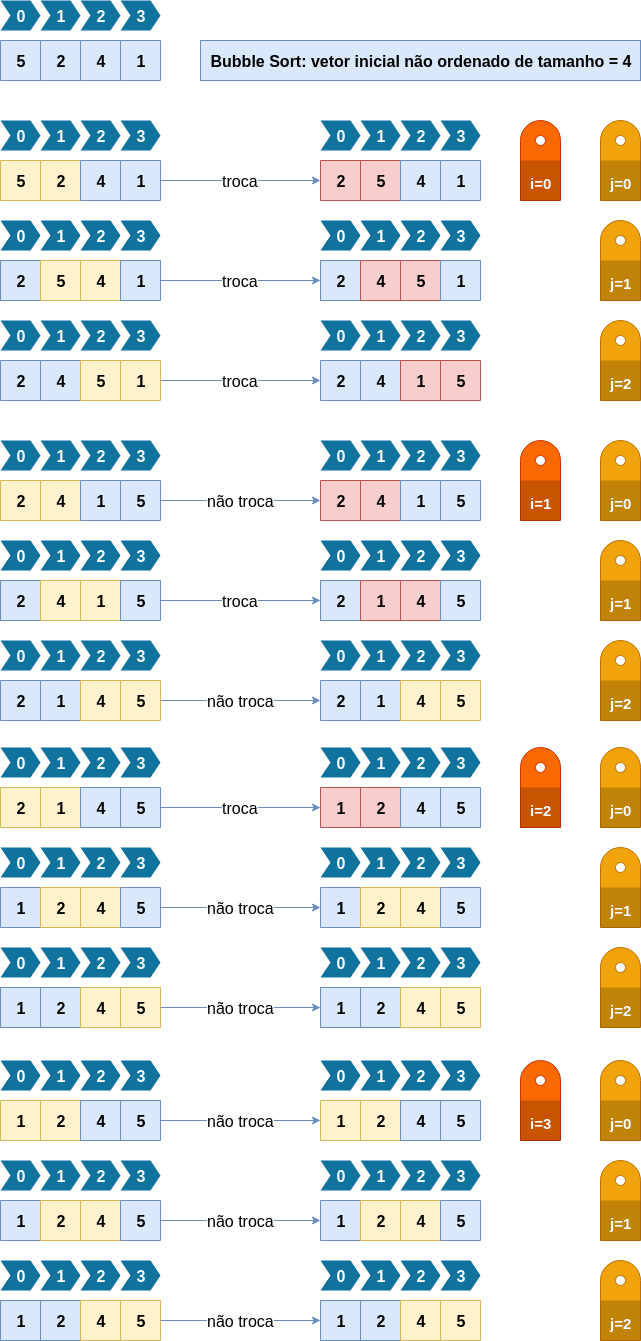
\includegraphics[width=.7\textwidth]{Pictures/BubbleSort}
	\caption[Bubble Sort]{Algoritmo \textit{Bubble Sort} para um vetor de tamanho 4.}
	\label{diaBubleSort}
\end{figure}

\subsection*{Exercícios}
\begin{enumerate}
	\item Atualizar a implementação do \textit{Bubble Sort} para executar as seguinte tarefa:
	\begin{itemize}
		\item executar o algoritmo com três vetores de entrada:
			\begin{enumerate}
				\item um vetor ordenado crescente de tamanho 100000 (cem mil)
				\item um vetor com números aleatórios de tamanho 100000 (cem mil)
				\item um vetor ordenado decrescente de tamanho 100000 (cem mil)
			\end{enumerate} 
		\item criar variáveis para contar a quantidade de comparações e quantidade de trocas;
	\end{itemize} 
	\item Criar gráficos para as três execuções comparando quantidade de comparações e quantidade de trocas e o tempo de execução;
\end{enumerate} 

\newpage
\subsection*{Selection Sort}
No algoritmo de ordenação por seleção (\textit{Selection Sort}) cada número do vetor, a partir do primeiro, é eleito e comparado com o menor número\footnote{Ou maior dependendo da ordenação desejada.} entre aqueles que estão à direita do eleito.
O  programa~\ref{SelectionSort} apresenta uma implementação em C do algoritmo \textit{Selection Sort} para um vetor de tamanho 4.
%, e a Figura~\ref{diaSelectionSort} ilustra seu funcionamento.
\lstinputlisting[language=C, caption={Implementação em C do algoritmo de ordenação Selection.}]{Code/Ordenacao/SelectionSort.c}\label{SelectionSort}
%\begin{figure}
%	\centering
%	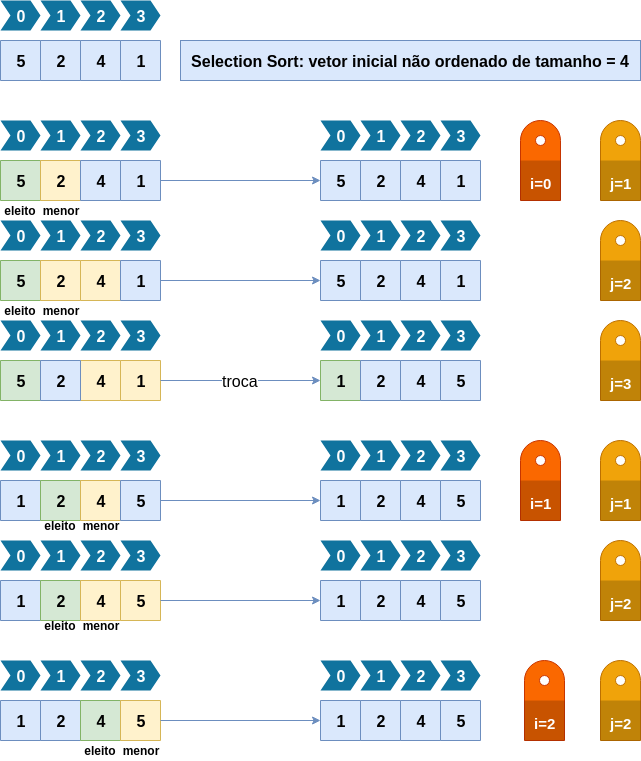
\includegraphics[width=.75\textwidth]{Pictures/SelectionSort}
%	\caption[Selection Sort]{Algoritmo \textit{Selection Sort} para um vetor de tamanho 4.}
%	\label{diaSelectionSort}
%\end{figure}

\subsection*{Exercícios}
\begin{enumerate}
	\item Atualizar a implementação do \textit{Selection Sort} para executar as seguinte tarefa:
	\begin{itemize}
		\item executar o algoritmo com três vetores de entrada:
		\begin{enumerate}
			\item um vetor ordenado crescente de tamanho 100000 (cem mil)
			\item um vetor com números aleatórios de tamanho 100000 (cem mil)
			\item um vetor ordenado decrescente de tamanho 100000 (cem mil)
		\end{enumerate} 
		\item criar variáveis para contar a quantidade de comparações e quantidade de trocas;
	\end{itemize} 
	\item Criar gráficos para as três execuções comparando quantidade de comparações e quantidade de trocas e o tempo de execução;
\end{enumerate} 
\newpage
\subsection*{Insertion Sort}
O algoritmo de ordenação por inserção (\textit{Insertion Sort}), funciona como uma mão de baralho onde você ordena suas cartas começando a comparação entre as duas primeiras.
No \textit{Insertion Sort}, é eleito o segundo elemento do vetor para iniciar a comparção. É percorrido o vetor de forma a garantir que todos os números à esquerda do eleito sejam menores que ele.
O programa~\ref{InsertionSort} apresenta uma implementação em C do algoritmo \textit{Insertion Sort} para um vetor de tamanho 4.
\lstinputlisting[language=C, caption={Implementação em C do algoritmo de ordenação Insertion Sort.}]{Code/Ordenacao/InsertionSort.c}\label{InsertionSort}
%\begin{figure}
%	\centering
%	\includegraphics[width=.75\textwidth]{Pictures/InsertionSort}
%	\caption[Selection Sort]{Algoritmo \textit{Selection Sort} para um vetor de tamanho 4.}
%	\label{diaInsertionSort}
%\end{figure}

\subsection*{Exercícios}
\begin{enumerate}
	\item Atualizar a implementação do \textit{Insertion Sort} para executar as seguinte tarefa:
	\begin{itemize}
		\item executar o algoritmo com três vetores de entrada:
		\begin{enumerate}
			\item um vetor ordenado crescente de tamanho 100000 (cem mil)
			\item um vetor com números aleatórios de tamanho 100000 (cem mil)
			\item um vetor ordenado decrescente de tamanho 100000 (cem mil)
		\end{enumerate} 
		\item criar variáveis para contar a quantidade de comparações e quantidade de trocas;
	\end{itemize} 
	\item Criar gráficos para as três execuções comparando quantidade de comparações e quantidade de trocas e o tempo de execução;
\end{enumerate} 
\newpage
\subsection*{Merge Sort}
O algoritmo de ordenação \textit{Merge Sort} a técnica de divisão e conquista, ou seja, o problema é dividido em subproblemas menores até que a solução para o subproblema seja simples.
As soluções dos subproblemas são combinadas para prover a solução do problema original.

No \textit{Merge Sort}, o vetor é dividido em partes iguais recursivamente até que haja apenas um elemento. Por exemplo se um vetor tem $n$ elementos, ele é divido em $n/2$, o resultado é novamente dividido por $2$ até que o vetor não seja mais divisível.
Os pares da última divisão são ordenados entre si assim como na volta recursiva montando o vetor original que estará então ordenado.
O programa~\ref{MergeSort} apresenta uma implementação em C do algoritmo \textit{Merge Sort} para um vetor de tamanho 4.
\lstinputlisting[language=C, caption={Implementação em C do algoritmo de ordenação Merge Sort.}]{Code/Ordenacao/MergeSort.c}\label{MergeSort}

\subsection*{Exercícios}
\begin{enumerate}
	\item Atualizar a implementação do \textit{Merge Sort} para executar as seguinte tarefa:
	\begin{itemize}
		\item executar o algoritmo com três vetores de entrada:
		\begin{enumerate}
			\item um vetor ordenado crescente de tamanho 100000 (cem mil)
			\item um vetor com números aleatórios de tamanho 100000 (cem mil)
			\item um vetor ordenado decrescente de tamanho 100000 (cem mil)
		\end{enumerate} 
		\item criar variáveis para contar a quantidade de comparações e quantidade de trocas;
	\end{itemize} 
	\item Criar gráficos para as três execuções comparando quantidade de comparações e quantidade de trocas e o tempo de execução;
\end{enumerate} 


\newpage
\subsection*{Quick Sort}
O algoritmo de ordenação \textit{Quick Sort} também utiliza a técnica de divisão e conquista.
No \textit{Quick Sort}, o vetor é dividido em duas partes recursivamente a partir de um pivô escolhido, até que não seja possível dividir mais. 
Os pares da última divisão são ordenados entre si assim na volta recursiva colocando todos os valores menores que o pivô no vetor à sua esquerda e todos os valores maiores que o pivô no vetor à sua direita.
Após esse procedimento o pivô estará ordenado em sua posição com relação os demais números.
O programa~\ref{QuickSort} apresenta uma implementação em C do algoritmo \textit{Quick Sort} para um vetor de tamanho 4.
\lstinputlisting[language=C, caption={Implementação em C do algoritmo de ordenação Quick Sort.}]{Code/Ordenacao/QuickSort.c}\label{QuickSort}

\subsection*{Exercícios}
\begin{enumerate}
	\item Atualizar a implementação do \textit{Quick Sort} para executar as seguinte tarefa:
	\begin{itemize}
		\item executar o algoritmo com três vetores de entrada:
		\begin{enumerate}
			\item um vetor ordenado crescente de tamanho 100000 (cem mil)
			\item um vetor com números aleatórios de tamanho 100000 (cem mil)
			\item um vetor ordenado decrescente de tamanho 100000 (cem mil)
		\end{enumerate} 
		\item criar variáveis para contar a quantidade de comparações e quantidade de trocas;
	\end{itemize} 
	\item Criar gráficos para as três execuções comparando quantidade de comparações e quantidade de trocas e o tempo de execução;
\end{enumerate} 
\section{Listas}\label{listas}

\section{Pilhas}\label{pilhas}

\section{Filas}\label{filas}

\section{Tabelas Hashing}\label{hashing}

\section{Árvores}\label{arvores}

\section{Grafos}\label{grafos}

\subsection{Busca em Grafos}

%----------------------------------------------------------------------------------------
%	CHAPTER X
%----------------------------------------------------------------------------------------
%------------------------------------------------
\chapterimage{06.jpg} % Chapter heading image
\chapter{Aplicações}\label{aplicacoes}
\vspace{6em}
\begin{flushright}
	\textit{\textcolor{white}{Um bonita citação...}}
\end{flushright}
\vspace{12em}



% ----------------------------------------------------------------------------------------
% 	BIBLIOGRAPHY
% ----------------------------------------------------------------------------------------
%----------------------------------------------------------------------------------------
%	CHAPTER X
%----------------------------------------------------------------------------------------
%------------------------------------------------
\chapterimage{07.jpg} % Chapter heading image
%\chapter*{Referências Bibliográficas}
%\bibliography{bibliography}
%\renewcommand\bibname{Referências Bibliográficas}

\chapter*{Referências Bibliográficas}\label{referencias}
\vspace{6em}
\begin{flushright}
	\textit{\textcolor{white}{Um bonita citação...}}
\end{flushright}
\vspace{12em}
%\addcontentsline{toc}{chapter}{\textcolor{verde}{Bibliography}}
%\section{Books}
%\addcontentsline{toc}{section}{Books}
%\printbibliography[heading=bibempty,type=book]
%\section{Articles}
%\addcontentsline{toc}{section}{Articles}
%\printbibliography[heading=bibempty,type=article]
\printbibliography[heading=bibempty]


%----------------------------------------------------------------------------------------

%----------------------------------------------------------------------------------------
%	INDEX
%----------------------------------------------------------------------------------------
%
%\cleardoublepage
%\phantomsection
%\setlength{\columnsep}{0.75cm}
%\addcontentsline{toc}{chapter}{\textcolor{verde}{Index}}
%\printindex


%----------------------------------------------------------------------------------------
%	CHAPTER X
%----------------------------------------------------------------------------------------
%------------------------------------------------
\chapterimage{08.jpg} % Chapter heading image
\chapter{Apêncice}\label{apendice}
\vspace{6em}
\begin{flushright}
	\textit{\textcolor{white}{}}
\end{flushright}
\vspace{12em}


\end{document}
